\documentclass[11pt,a4paper]{article}
\usepackage{kotex}
\usepackage[margin=18mm]{geometry}
\usepackage{amsmath,booktabs,array,graphicx,needspace}
\usepackage{pgfplots}
\pgfplotsset{compat=1.18}
\usepgfplotslibrary{groupplots}
\usepackage[hidelinks]{hyperref}
\usepackage{xurl}
\setlength{\parindent}{0pt}
\setlength{\parskip}{6pt}
\setlength{\emergencystretch}{1em}
\renewcommand{\arraystretch}{1.18}
\begin{document}
{\LARGE\bfseries zkDPP 논문용 실험 결과 초안}\par\medskip
\section*{실험 환경}
\begin{center}\small\begin{tabular}{@{}ll@{}}\toprule
        \textbf{항목}    & \textbf{설정}                                           \\
        \midrule
        Host PC        & MacBook Pro (MacBookPro18,1)                          \\
        Host OS        & macOS 26.3 (25D125)                                   \\
        CPU            & Apple M1 Pro, 10 cores (8 Performance + 2 Efficiency) \\
        Host Memory    & 32 GB                                                 \\
        \midrule
        Circuit 라이브러리  & gnark 0.15.0 / gnark-crypto 0.20.1                    \\
        Proof system   & PLONK-KZG / BLS12-381 / Jubjub                        \\
        Hash           & Poseidon2                                             \\
        Blokchain Node & Anvil 1.7.1                                           \\
        Contract 컴파일러  & Solidity 0.8.30                                       \\
        EVM            & Prague                                                \\
        \bottomrule\end{tabular}\end{center}

\needspace{8\baselineskip}\section*{1. 공급망 Event별 실행 비용}
\textbf{실험을 진행한 이유}\newline
zkDPP의 Event는 공급망 동작에 더해 Proof를 검증하고 AuditRecord도 기록합니다.\newline
이 작업들을 모두 수행하면, Event 하나를 실행하는 데 비용과 시간이 너무 많이 드는 것은 아닐까요?

\textbf{실험 목적}\newline
9개 Event의 Constraints, 실제 transaction Gas, E2E를 측정합니다.\newline

\textbf{표·그래프 구성}\newline
Event 종류는 연속적인 증가 변수가 아니므로 정확한 값을 비교할 수 있는 표를 사용합니다.\newline

\textbf{고정 조건}\newline
모든 Supply Chain Event는 AuditRecord를 기록합니다.\newline
State는 3개이며 Process의 입출력은 2$\rightarrow$1입니다.\newline

\begin{center}\small\begin{tabular}{@{}lrrr@{}}\toprule
        \textbf{Event} & \textbf{Constraints} & \textbf{Gas} & \textbf{E2E (ms)} \\
        \midrule
        Entry          & 18,115               & 2,258,715    & 770.834           \\
        Transfer       & 49,883               & 3,577,414    & 1,464.369         \\
        Proceed        & 35,858               & 1,784,082    & 1,278.965         \\
        Recall         & 35,987               & 1,785,084    & 1,250.315         \\
        Merge          & 51,543               & 1,888,301    & 1,361.248         \\
        Split          & 48,608               & 2,730,046    & 1,497.729         \\
        Process        & 55,402               & 1,866,617    & 1,335.974         \\
        Exit           & 27,940               & 534,277      & 674.484           \\
        Issue          & 35,957               & 678,565      & 1,225.264         \\
        \bottomrule\end{tabular}\end{center}

\par\noindent\begin{minipage}{\linewidth}
    \textbf{해석}\newline
    비용의 핵심 증가 원인은 다음과 같습니다.\newline

    \textbf{Constraints}: Merkle Path 검증 + Encrypted AuditRecord 검증 + State 관계 검증 + cm/nf 계산\newline
    \textbf{Gas}: Merkle Tree Update + Proof 검증 +  AuditRecord 저장 비용\newline

    Merkle Path 1회 검증, Merkle Tree 2회 Update를 진행하는 Transfer를 대표적인 Event로 선택해, Constraints와 Gas 소비를 분석합니다.\newline

    Audit과 관련된 추가 비용은 2.1절에서 추가로 분석했습니다.\newline

    \begin{center}\small
    \begin{minipage}[t]{0.48\linewidth}
        \centering\textbf{(a) Merkle Path Verify}\par\smallskip
        \begin{tabular}{@{}c p{0.76\linewidth}@{}}\toprule
            \textbf{횟수} & \textbf{Event}                                           \\
            \midrule
            0           & Entry                                                    \\
            1           & Transfer / Proceed / Recall\newline Split / Exit / Issue \\
            2           & Merge / Process                                          \\
            \bottomrule
        \end{tabular}
    \end{minipage}\hfill
    \begin{minipage}[t]{0.48\linewidth}
        \centering\textbf{(b) Merkle Tree Update}\par\smallskip
        \begin{tabular}{@{}c p{0.76\linewidth}@{}}\toprule
            \textbf{횟수} & \textbf{Event}                                   \\
            \midrule
            0           & Exit / Issue                                     \\
            1           & Entry / Proceed / Recall\newline Merge / Process \\
            2           & Transfer / Split                                 \\
            \bottomrule
        \end{tabular}
    \end{minipage}
\end{center}

    \noindent\begin{minipage}[t]{0.48\linewidth}
        \vspace{0pt}\centering\small
        \textbf{Transfer의 Constraints 구성}\par\smallskip
\begin{tabular}{@{}p{0.62\linewidth}r@{}}\toprule
    \textbf{비용 요인}           & \textbf{Constraints} \\
    \midrule
    Merkle Path 검증           & 9,825                \\
    Encrypted AuditRecord 검증 & 14,238               \\
    State 범위·배분 등 검증         & 17,994               \\
    cm/nf·owner address 계산   & 7,826                \\
    \midrule
    \textbf{Transfer 합계}     & \textbf{49,883}      \\
    \bottomrule
\end{tabular}\par\smallskip

    \end{minipage}\hfill
    \begin{minipage}[t]{0.48\linewidth}
        \vspace{0pt}\centering\small
        \textbf{Transfer의 Gas Cost 구성}\par\smallskip
\begin{tabular}{@{}lr@{}}\toprule
    \textbf{비용 요인}       & \textbf{Gas}       \\
    \midrule
    Merkle Tree Hash 계산  & 1,422,404          \\
    Merkle Tree 조회·저장    & 1,276,500          \\
    Proof 검증 호출          & 335,007            \\
    Audit 추가 비용          & 356,146            \\
    nf·cm·rv 조회·저장       & 68,700             \\
    calldata 등 기타 비용     & 118,657            \\
    \midrule
    \textbf{Transfer 합계} & \textbf{3,577,414} \\
    \bottomrule
\end{tabular}\par\smallskip

    \end{minipage}
\end{minipage}\par

\clearpage
\needspace{8\baselineskip}\section*{2. Audit 추가 비용과 Auditor 수행 비용}

\needspace{6\baselineskip}\subsection*{2.1 Event별 Audit 추가 비용}
\textbf{실험을 진행한 이유}\newline
zkDPP의 Event는 Auditing에 필요한 정보를 암호화해 기록합니다.\newline
Audit이 없는 같은 Event보다 Constraints와 Gas가 크게 증가하는 것은 아닐까요?

\textbf{표·그래프 구성}\newline
입력·State·권한·Tree 조건을 맞춘 Audit X/O 막대를 Event별로 나란히 배치합니다.\newline
Constraints와 Gas는 단위가 다르므로 그래프를 분리하고, 표에는 각각의 증가량을 표시합니다.


\par\noindent\begin{minipage}{\linewidth}
    \centering\resizebox{\linewidth}{!}{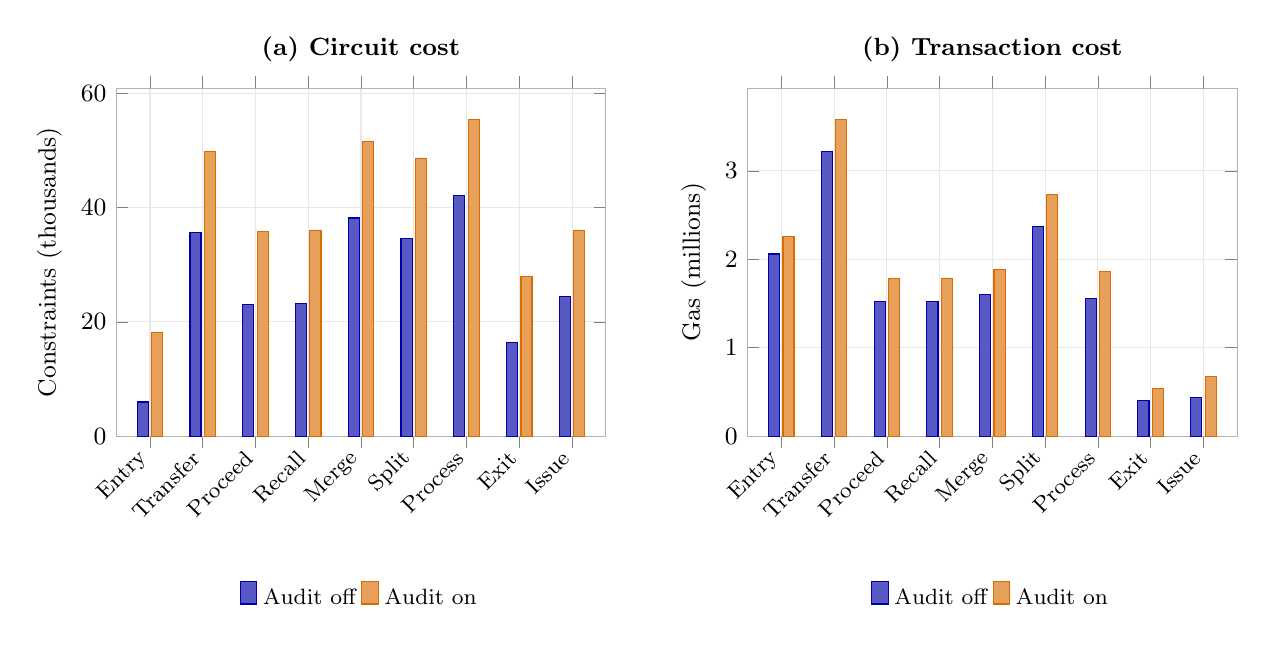
\begin{tikzpicture}
            \begin{groupplot}[group style={group size=2 by 1,horizontal sep=1.8cm},width=7.8cm,height=6.0cm,grid=major,major grid style={gray!18},axis line style={gray!60},tick label style={font=\small},label style={font=\small},title style={font=\small\bfseries},legend style={font=\footnotesize,draw=none},scaled ticks=false]
                \nextgroupplot[ybar,single ybar legend,ymin=0,ylabel={Constraints (thousands)},title={(a) Circuit cost},symbolic x coords={Entry,Transfer,Proceed,Recall,Merge,Split,Process,Exit,Issue},xtick=data,x tick label style={rotate=45,anchor=east,font=\footnotesize},enlarge x limits=0.08,legend style={at={(0.5,-0.40)},anchor=north,legend columns=2}]
                \addplot+[ybar,bar width=4pt,bar shift=-2.6pt,draw=blue!65!black,fill=blue!65!black!65,mark=none] coordinates {(Entry,5.98) (Transfer,35.645) (Proceed,23.123) (Recall,23.252) (Merge,38.208) (Split,34.671) (Process,42.067) (Exit,16.407) (Issue,24.424)};
                \addplot+[ybar,bar width=4pt,bar shift=2.6pt,draw=orange!85!black,fill=orange!85!black!65,mark=none] coordinates {(Entry,18.115) (Transfer,49.883) (Proceed,35.858) (Recall,35.987) (Merge,51.543) (Split,48.608) (Process,55.402) (Exit,27.94) (Issue,35.957)};
                \legend{Audit off,Audit on}

                \nextgroupplot[ybar,single ybar legend,ymin=0,ylabel={Gas (millions)},title={(b) Transaction cost},symbolic x coords={Entry,Transfer,Proceed,Recall,Merge,Split,Process,Exit,Issue},xtick=data,x tick label style={rotate=45,anchor=east,font=\footnotesize},enlarge x limits=0.08,legend style={at={(0.5,-0.40)},anchor=north,legend columns=2}]
                \addplot+[ybar,bar width=4pt,bar shift=-2.6pt,draw=blue!65!black,fill=blue!65!black!65,mark=none] coordinates {(Entry,2.059123) (Transfer,3.221268) (Proceed,1.519228) (Recall,1.520722) (Merge,1.599289) (Split,2.373759) (Process,1.557348) (Exit,0.403572) (Issue,0.438706)};
                \addplot+[ybar,bar width=4pt,bar shift=2.6pt,draw=orange!85!black,fill=orange!85!black!65,mark=none] coordinates {(Entry,2.258715) (Transfer,3.577414) (Proceed,1.784082) (Recall,1.785084) (Merge,1.888301) (Split,2.730046) (Process,1.866617) (Exit,0.534277) (Issue,0.678565)};
                \legend{Audit off,Audit on}

            \end{groupplot}
        \end{tikzpicture}}
    \par\smallskip{\small 그림 1. 동일 Event의 Audit 유무에 따른 비용 비교.}\par\medskip
    \par\medskip\noindent
    \begin{minipage}[t]{.49\linewidth}\centering
        {\small\setlength{\tabcolsep}{7pt}\renewcommand{\arraystretch}{1.12}
            \textbf{(a) Constraints}\par\smallskip
            \begin{tabular}{@{}lrrr@{}}\toprule
                \textbf{Event} & \textbf{Audit X} & \textbf{Audit O} & \textbf{증가량}    \\
                \midrule
                Entry          & 5,980            & 18,115           & \textbf{12,135} \\
                Transfer       & 35,645           & 49,883           & \textbf{14,238} \\
                Proceed        & 23,123           & 35,858           & \textbf{12,735} \\
                Recall         & 23,252           & 35,987           & \textbf{12,735} \\
                Merge          & 38,208           & 51,543           & \textbf{13,335} \\
                Split          & 34,671           & 48,608           & \textbf{13,937} \\
                Process        & 42,067           & 55,402           & \textbf{13,335} \\
                Exit           & 16,407           & 27,940           & \textbf{11,533} \\
                Issue          & 24,424           & 35,957           & \textbf{11,533} \\
                \bottomrule\end{tabular}}
    \end{minipage}\hfill
    \begin{minipage}[t]{.49\linewidth}\centering
        {\small\setlength{\tabcolsep}{7pt}\renewcommand{\arraystretch}{1.12}
            \textbf{(b) Gas}\par\smallskip
            \begin{tabular}{@{}lrrr@{}}\toprule
                \textbf{Event} & \textbf{Audit X} & \textbf{Audit O} & \textbf{증가량}     \\
                \midrule
                Entry          & 2,059,123        & 2,258,715        & \textbf{199,592} \\
                Transfer       & 3,221,268        & 3,577,414        & \textbf{356,146} \\
                Proceed        & 1,519,228        & 1,784,082        & \textbf{264,854} \\
                Recall         & 1,520,722        & 1,785,084        & \textbf{264,362} \\
                Merge          & 1,599,289        & 1,888,301        & \textbf{289,012} \\
                Split          & 2,373,759        & 2,730,046        & \textbf{356,287} \\
                Process        & 1,557,348        & 1,866,617        & \textbf{309,269} \\
                Exit           & 403,572          & 534,277          & \textbf{130,705} \\
                Issue          & 438,706          & 678,565          & \textbf{239,859} \\
                \bottomrule\end{tabular}}
    \end{minipage}
    \par\medskip
\end{minipage}\par\medskip


\textbf{해석}

\textbf{Constraints 증가량은 약 1.1만--1.4만 개로, Event별로 비슷합니다.}\newline
Encrypted AuditRecord 검증에 필요한 R·Z의 scalar multiplication 두 번이 큰 공통 비용을 만듭니다.\newline
암호화할 Field 수와 출력 nf·rvnf 계산에 따라 나머지 증가량이 달라집니다.

\textbf{Gas 증가량은 약 13만--36만이며, Traceability 정보를 기록하는 SSTORE 비용이 크게 반영됩니다.}\newline
Contract는 Event가 만든 cm·rv·h마다 해당 Event의 AuditRecord ID를 기록합니다.\newline
따라서 출력 cm·rv·h와 AuditRecord에 담는 암호화 값이 많아질수록 SSTORE 횟수도 증가합니다.

\par\medskip\noindent\begin{minipage}{\linewidth}
    \begin{minipage}[t]{0.48\linewidth}
        \centering\small
        \textbf{Transfer의 Audit 추가 Constraints}\par\smallskip
        \begin{tabular}{@{}lr@{}}\toprule
            \textbf{비용 요인}            & \textbf{Constraints} \\
            \midrule
            R·Z scalar multiplication & 8,611                \\
            키·mask 계산                 & 2,399                \\
            난수·암호문 등 검증               & 1,723                \\
            출력 nf·rvnf 계산             & 1,505                \\
            \midrule
            \textbf{합계}               & \textbf{14,238}      \\
            \bottomrule
        \end{tabular}
    \end{minipage}\hfill
    \begin{minipage}[t]{0.48\linewidth}
        \centering\small
        \textbf{Transfer의 Audit 추가 Gas}\par\smallskip
        \begin{tabular}{@{}lr@{}}\toprule
            \textbf{비용 요인}          & \textbf{Gas}     \\
            \midrule
            % AuditRecord 본문 및 cm·rv의 AuditRecord ID 기록을 합산.
            AuditRecord SSTORE      & 324,100          \\
            Proof 검증 호출 증가분         & 4,585            \\
            SLOAD·calldata 등 기타 증가분 & 27,461           \\
            \midrule
            \textbf{합계}             & \textbf{356,146} \\
            \bottomrule
        \end{tabular}
    \end{minipage}
\end{minipage}\par\medskip



\clearpage
\needspace{6\baselineskip}\subsection*{2.2 Tracing·Freeze 비용}
\textbf{실험을 진행한 이유}\newline
Tracing은 연결된 AuditRecord를 조회하고 복호화해야 합니다.\newline
공급망이 길어져 방문할 기록이 많아지면, 추적에 너무 오래 걸리는 것은 아닐까요?\newline
Freeze도 대상마다 transaction을 실행하므로, 동결 대상이 많아지면 시간과 Gas 부담이 커지는 것은 아닐까요?

\textbf{표·그래프 구성}\newline
Tracing과 Freeze를 병렬로 배치하고, 같은 시간 단위와 로그축 범위로 비교합니다.\newline
이 Split 시나리오에서는 방문 AuditRecord 수와 Freeze 대상 수가 각각 10·100·1,000개입니다.

\textbf{측정 범위}\newline
Tracing은 기록 조회·복호화·연결 탐색 시간입니다.\newline
Freeze는 제출 전 상태 검사부터 개별 동결 transaction·최종 상태 확인까지입니다.\newline

\par\noindent\begin{minipage}{\linewidth}
    \centering
    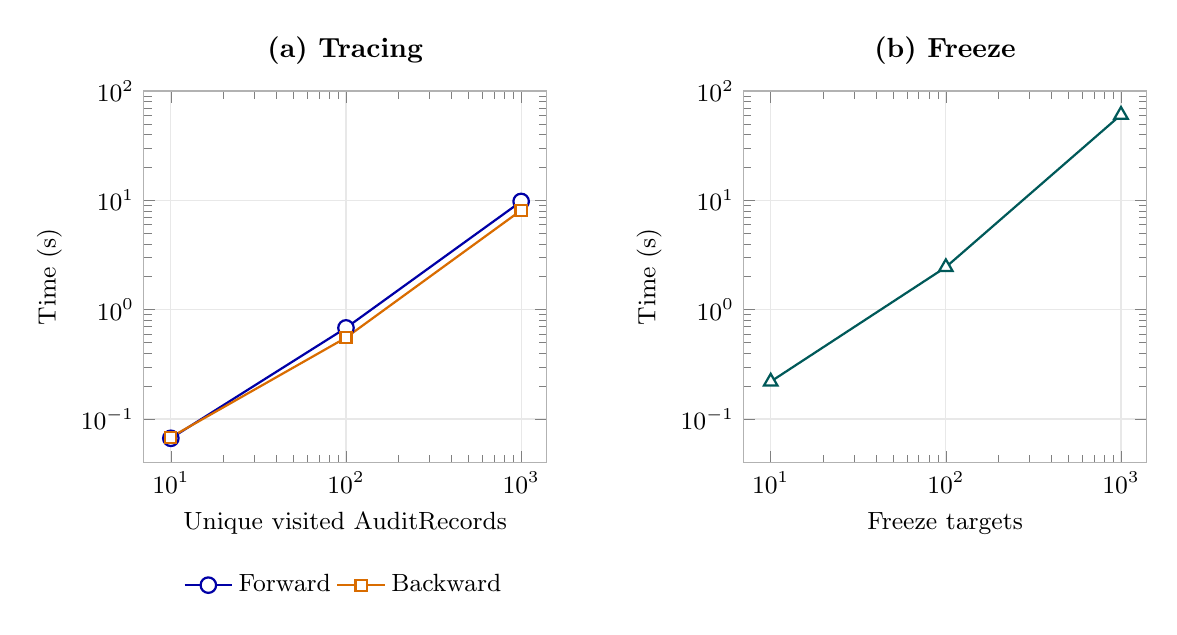
\begin{tikzpicture}
        \begin{groupplot}[group style={group size=2 by 1,horizontal sep=2.5cm},width=6.7cm,height=6.3cm,grid=major,major grid style={gray!18},axis line style={gray!60},tick label style={font=\small},label style={font=\small},title style={font=\bfseries},scaled ticks=false,xmode=log,ymode=log,xmin=7,xmax=1400,ymin=0.04,ymax=100,xtick={10,100,1000},ytick={0.1,1,10,100},ylabel={Time (s)},legend style={at={(0.5,-0.27)},anchor=north,legend columns=2,font=\small,draw=none}]
            \nextgroupplot[title={(a) Tracing},xlabel={Unique visited AuditRecords}]
            \addplot+[color=blue!65!black,mark=*,mark size=2.8pt,mark options={solid,fill=white},thick] coordinates {(10,0.066552708) (100,0.680694458) (1000,9.760276625)};
            \addplot+[color=orange!85!black,mark=square*,mark size=2pt,mark options={solid,fill=white},thick] coordinates {(10,0.068203167) (100,0.55413275) (1000,8.102012541)};
            \legend{Forward,Backward}
            \nextgroupplot[title={(b) Freeze},xlabel={Freeze targets}]
            \addplot+[color=teal!70!black,mark=triangle*,mark size=2.8pt,mark options={solid,fill=white},thick] coordinates {(10,0.219802208) (100,2.448003417) (1000,60.539842)};
        \end{groupplot}
    \end{tikzpicture}
    \par\medskip{\small 그림 2. 같은 공급망 시나리오의 Tracing·Freeze 시간.}\par\medskip
    \begin{minipage}[t]{0.48\linewidth}
        \centering\small\setlength{\tabcolsep}{6pt}
        \textbf{Tracing}\par\smallskip
        \begin{tabular}{@{}rrr@{}}\toprule
            \shortstack{\textbf{Visited}\\\textbf{AuditRecords}} & \shortstack{\textbf{Forward}\\\textbf{(s)}} & \shortstack{\textbf{Backward}\\\textbf{(s)}} \\
            \midrule
            10                                                   & 0.067                                       & 0.068                                        \\
            100                                                  & 0.681                                       & 0.554                                        \\
            1,000                                                & 9.760                                       & 8.102                                        \\
            \bottomrule
        \end{tabular}
    \end{minipage}\hfill
    \begin{minipage}[t]{0.48\linewidth}
        \centering\small\setlength{\tabcolsep}{7pt}
        \textbf{Freeze}\par\smallskip
        \begin{tabular}{@{}rr@{}}\toprule
            \textbf{Freeze targets} & \textbf{Time (s)}               \\
            \midrule
            10                      & 0.220                           \\
            100                     & 2.448                           \\
            1,000                   & 60.540                          \\
            \midrule
            \multicolumn{2}{@{}c@{}}{\textbf{Gas per target: 49,434}} \\
            \bottomrule
        \end{tabular}
    \end{minipage}
\end{minipage}\par\medskip


\clearpage
\needspace{8\baselineskip}\section*{3. zkTransfer와 Voucher 전달 Tradeoff 비용}
\textbf{실험을 진행한 이유}\newline
zkTransfer는 한 번에 Receiver Note를 만들지만, Voucher 전달은 Transfer와 Proceed 두 단계가 필요합니다.\newline
Proof와 transaction이 하나씩 늘어나면 Gas가 당연히 증가할꺼라 생각해요.\newline
zkTransfer를 조금 변경한 SharedSecret 구조로도 Traceability는 제공할 수 있어보이는데, 왜 Voucher가 필요할까요?

\textbf{SharedSecret zkTransfer란?}\newline
기존 zkTransfer는 owner secret sk를 사용해 nf=H(cm, sk)를 계산합니다.\newline
SharedSecret zkTransfer는 이를 shared secret `o`로 계산하도록 변경한 구조입니다.\newline
Sender와 Receiver가 opening을 공유하므로, Sender도 Receiver Note의 nf를 계산할 수 있습니다.\newline
Receiver Note의 nf를 계산할 수 있으면, Receiver가 Note를 소비하는 시점을 식별할 수 있는 문제가 있습니다.\newline
이후로는 sharedSecret zkTrasnfer를 zkTransfer\textsuperscript{2}로 표기하겠습니다.

\textbf{Vocher를 도입함으로써 얻는 장점}

\textbf{1. Receiver 수령 전 Sender의 Recall}\newline
Receiver가 Proceed하기 전에는 Sender가 허용된 기한 안에서 Recall할 수 있습니다.\newline
Sender가 직접 Note를 회수할 수 있다는 점이 중요합니다.\newline

\textbf{2. Sender에게는 후속 소비를 숨기고, Auditor에게는 추적을 허용}\newline
SharedSecret zkTransfer에서는 Sender도 Receiver Note의 nf를 계산해 후속 소비를 식별할 수 있습니다.\newline
Voucher 방식에서는 Receiver가 Voucher를 소비한 시점을 알지만, 실제로 Note를 소비한 시점을 알 수 없습니다.\newline
Sender는 Voucher의 nf를 계산할 수 있으므로, Sender가 Note를 소비 할 때 Receiver의 rvnf를 AuditRecord에 등록할 수 있습니다.\newline
Auditor는 암호화된 rvnf를 복원해 Forward Tracing을 수행할 수 있습니다.\newline

\textbf{비교 조건}\newline
\textbf{zkTransfer\textsuperscript{1}:} Audit 없는 owner secret 기반 zkTrasnfer입니다.\newline
\textbf{zkTransfer\textsuperscript{2}:} Audit을 지원하지만 Sender도 후속 소비를 식별할 수 있는 직접 전달입니다.\newline
\textbf{zkDPP:} Audit을 포함한 Transfer $\rightarrow$ Recall 경로의 합계입니다.

표는 세 방식의 기능과 Gas를 비교합니다.\newline
Recall 경로는 정상 수령 경로와 결과가 다르며, Audit 조건도 달라 Voucher만의 순수 추가 비용은 아닙니다.

\begin{center}\small\begin{tabular}{@{}lcccr@{}}\toprule
        \textbf{전달 방식}                & \textbf{Traceability} & \textbf{Privacy} & \textbf{Recall} & \textbf{총 Gas} \\
        \midrule
        zkTransfer\textsuperscript{1} & X                     & O                & X               & 2,366,228      \\
        zkTransfer\textsuperscript{2} & O                     & $\triangle$      & X               & 2,724,242      \\
        zkDPP Transfer                & O                     & O                & O               & 5,362,498      \\
        \bottomrule\end{tabular}\par\smallskip
    $\triangle$: Sender가 Receiver의 후속 소비 시점을 식별할 수 있습니다.
\end{center}


\textbf{Azeroth의 zkTransfer와 총 Gas에서 크게 차이나는 이유}\newline
Azeroth의 zkTrasnfer의 총 Gas는 1,555,957로 실험한 zkTransfer\textsuperscript{1}와 총 Gas가 크게 차이납니다.\newline
Azeroth의 zkTransfer에서는 Sender의 잔여분을 암호화 계정 잔액인 ENA에 보관합니다.\newline
zkDPP에서 사용하는 zkTransfer\textsuperscript{1}는 Sender의 잔여분을 새로운 Note로 생성하여 Note Tree에 등록하고, address를 Sender로 지정합니다.
Balance 방식과 UTXO 방식의 차이로 인해 총 Gas 소비량에서 차이가 발생합니다.\newline

\clearpage
\needspace{8\baselineskip}\section*{4. Process 입출력 cm 수에 따른 비용}
\textbf{실험을 진행한 이유}\newline
공정에 따라 여러 원료를 투입하거나 제품·부산물 생산이 많은 경우가 있습니다. Event별 실행 비용에서 Process는 2-to-1으로 작성되어 있습니다.\newline
입력·출력 cm 수가 늘어나면, Process의 비용이 크게 증가하는 것은 아닐까요?

\textbf{실험 목적·범위}\newline
공정의 입력·출력 개수에 따른 Constraints와 Gas의 변화 경향을 확인합니다.\newline
모든 산업별 공정을 구현하는 대신, 기존 POC의 Sustainability Claim을 증명하기 위한 State로 범위를 제한해 경향성을 파악합니다.

\textbf{통제 조건}\newline
입출력 개수의 영향을 분리하기 위해 입력 State의 합(320,30,231)과 출력 State의 합(300,30,261)을 고정합니다.\newline
출력 N=1에서 입력 M을 늘리고 입력 M=2에서 출력 N을 늘립니다.

\textbf{표·그래프 구성}\newline
입력 증가와 출력 증가의 영향을 구분하기 위해 두 묶음의 그래프를 사용합니다.\newline
각 그래프의 왼쪽 축은 Constraints, 오른쪽 축은 Gas이며 색으로 구분합니다.\newline
두 그래프의 축 범위는 같게 유지하고, 아래 표에 정확한 수치를 제공합니다.


\noindent\begin{minipage}[t]{0.48\linewidth}
    \vspace{0pt}
    \par\noindent\begin{minipage}{\linewidth}
    \centering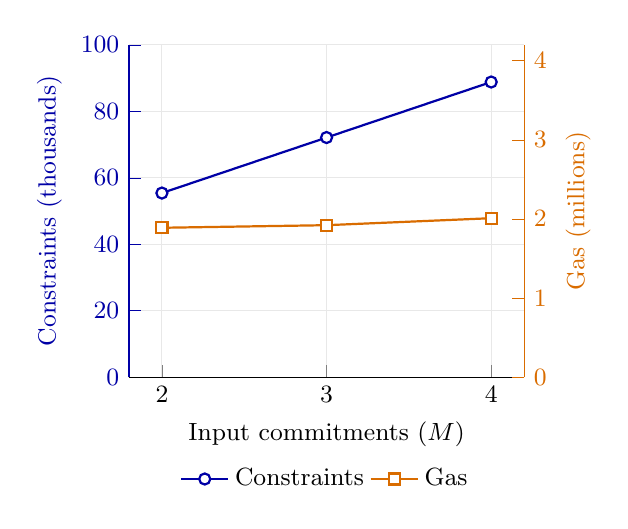
\begin{tikzpicture}
        \begin{axis}[width=6.6cm,height=5.8cm,xmin=1.8,xmax=4.2,xtick={2,3,4},scaled ticks=false,tick label style={font=\small},label style={font=\small},axis y line*=left,axis x line*=bottom,ymin=0,ymax=100,ytick={0,20,40,60,80,100},xlabel={Input commitments ($M$)},ylabel={Constraints (thousands)},y axis line style={blue!65!black},y tick style={blue!65!black},yticklabel style={blue!65!black},ylabel style={blue!65!black},grid=major,major grid style={gray!18},legend style={at={(0.5,-0.24)},anchor=north,legend columns=2,draw=none,font=\small}]
            \addplot[color=blue!65!black,mark=*,mark options={fill=white},thick] coordinates {(2,55.402) (3,72.116) (4,88.832)};
            \addlegendentry{Constraints}
            \addlegendimage{color=orange!85!black,mark=square*,mark options={fill=white},thick}
            \addlegendentry{Gas}
        \end{axis}
        \begin{axis}[width=6.6cm,height=5.8cm,xmin=1.8,xmax=4.2,xtick={2,3,4},scaled ticks=false,tick label style={font=\small},label style={font=\small},axis y line*=right,axis x line=none,ymin=0,ymax=4.2,ytick={0,1,2,3,4},ylabel={Gas (millions)},y axis line style={orange!85!black},y tick style={orange!85!black},yticklabel style={orange!85!black},ylabel style={orange!85!black}]
            \addplot[color=orange!85!black,mark=square*,mark options={fill=white},thick] coordinates {(2,1.887935) (3,1.920611) (4,2.009039)};
        \end{axis}
    \end{tikzpicture}
    \par\smallskip{\small 그림 3. 입력 수 증가 (N=1).}\par\medskip
    \par\medskip\noindent
    \begin{center}
        {\small\setlength{\tabcolsep}{7pt}\renewcommand{\arraystretch}{1.12}
            \textbf{Outputs N=1}\par\smallskip
            \begin{tabular}{@{}lrr@{}}\toprule
                \textbf{Input M} & \textbf{Constraints} & \textbf{Gas} \\
                \midrule
                2                & 55,402               & 1,887,935    \\
                3                & 72,116               & 1,920,611    \\
                4                & 88,832               & 2,009,039    \\
                \bottomrule\end{tabular}}
    \end{center}
    \par\medskip
\end{minipage}\par\medskip

\end{minipage}\hfill
\begin{minipage}[t]{0.48\linewidth}
    \vspace{0pt}
    \par\noindent\begin{minipage}{\linewidth}
    \centering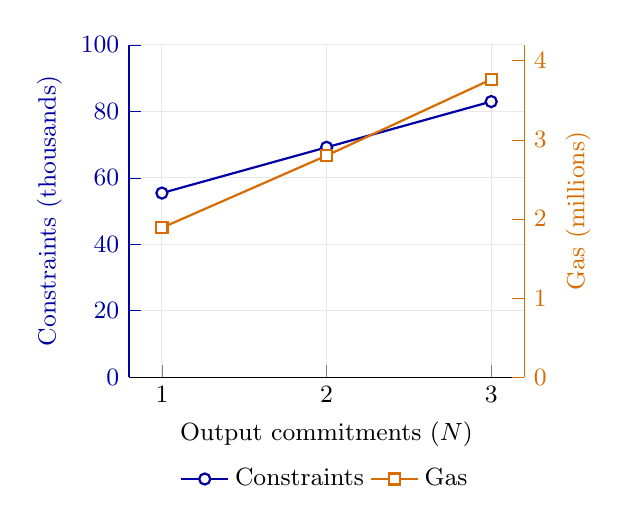
\begin{tikzpicture}
        \begin{axis}[width=6.6cm,height=5.8cm,xmin=0.8,xmax=3.2,xtick={1,2,3},scaled ticks=false,tick label style={font=\small},label style={font=\small},axis y line*=left,axis x line*=bottom,ymin=0,ymax=100,ytick={0,20,40,60,80,100},xlabel={Output commitments ($N$)},ylabel={Constraints (thousands)},y axis line style={blue!65!black},y tick style={blue!65!black},yticklabel style={blue!65!black},ylabel style={blue!65!black},grid=major,major grid style={gray!18},legend style={at={(0.5,-0.24)},anchor=north,legend columns=2,draw=none,font=\small}]
            \addplot[color=blue!65!black,mark=*,mark options={fill=white},thick] coordinates {(1,55.402) (2,69.172) (3,82.944)};
            \addlegendentry{Constraints}
            \addlegendimage{color=orange!85!black,mark=square*,mark options={fill=white},thick}
            \addlegendentry{Gas}
        \end{axis}
        \begin{axis}[width=6.6cm,height=5.8cm,xmin=0.8,xmax=3.2,xtick={1,2,3},scaled ticks=false,tick label style={font=\small},label style={font=\small},axis y line*=right,axis x line=none,ymin=0,ymax=4.2,ytick={0,1,2,3,4},ylabel={Gas (millions)},y axis line style={orange!85!black},y tick style={orange!85!black},yticklabel style={orange!85!black},ylabel style={orange!85!black}]
            \addplot[color=orange!85!black,mark=square*,mark options={fill=white},thick] coordinates {(1,1.887935) (2,2.800596) (3,3.763779)};
        \end{axis}
    \end{tikzpicture}
    \par\smallskip{\small 그림 4. 출력 수 증가 (M=2).}\par\medskip
    \par\medskip\noindent
    \begin{center}
        {\small\setlength{\tabcolsep}{7pt}\renewcommand{\arraystretch}{1.12}
            \textbf{Inputs M=2}\par\smallskip
            \begin{tabular}{@{}lrr@{}}\toprule
                \textbf{Output N} & \textbf{Constraints} & \textbf{Gas} \\
                \midrule
                1                 & 55,402               & 1,887,935    \\
                2                 & 69,172               & 2,800,596    \\
                3                 & 82,944               & 3,763,779    \\
                \bottomrule\end{tabular}}
    \end{center}
    \par\medskip
\end{minipage}\par\medskip

\end{minipage}


\clearpage
\needspace{8\baselineskip}\section*{5. k-of-n Master Key 복구 비용}
\textbf{실험을 진행한 이유}\newline
Auditor는 Committee로부터 전달받은 k개의 share로 Master Key를 복구합니다.\newline
k값에 따라서 복구 시간이 얼마나 늘어나나요?

\textbf{측정 범위}\newline
Committee의 공개키와 위원별 public share는 사전에 검증해 보관합니다.\newline
받은 k개 share의 검증, Lagrange 보간, 복구한 키의 공개키 일치 확인을 측정합니다.\newline
키 생성·DKG·통신·승인 대기는 제외합니다.

\textbf{비교 조건}\newline
Committee n=10을 고정하고 share k를 2·3·5·7·10개로 늘립니다.\newline
각 case는 warm-up 후 공식 1회 측정하며, 내부 1,000회 복구의 평균 시간을 표시합니다.

\par\noindent\begin{minipage}{\linewidth}
    \centering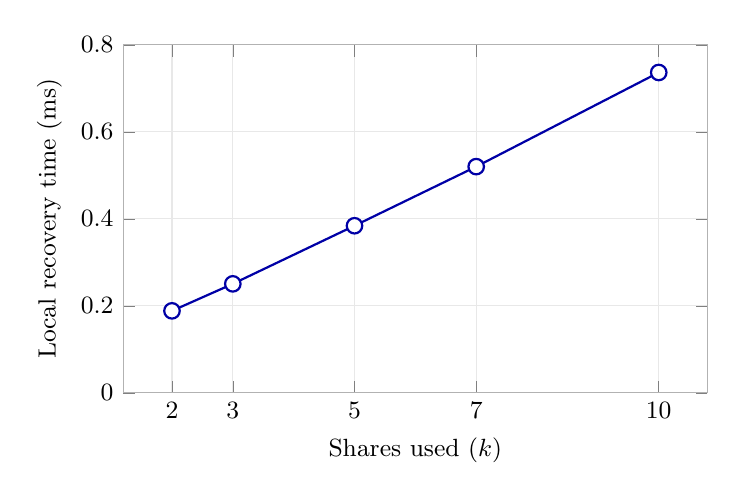
\begin{tikzpicture}
        \begin{axis}[width=9cm,height=6cm,grid=major,major grid style={gray!18},axis line style={gray!60},tick label style={font=\small},label style={font=\small},scaled ticks=false,xlabel={Shares used ($k$)},ylabel={Local recovery time (ms)},xtick={2,3,5,7,10},ymin=0,ymax=0.8]
            \addplot[color=blue!65!black,mark=*,mark size=2.8pt,mark options={fill=white},thick] coordinates {(2,0.188436) (3,0.250553334) (5,0.384199667) (7,0.520116083) (10,0.736622708)};
        \end{axis}
    \end{tikzpicture}
    \par\smallskip{\small 그림 5. Committee n=10에서 share k 증가에 따른 Master Key 복구 시간.}\par\medskip
    {\small\setlength{\tabcolsep}{7pt}
        \begin{tabular}{@{}rr@{}}\toprule
            \textbf{share k} & \textbf{복구 시간 (ms)} \\
            \midrule
            2                & 0.188               \\
            3                & 0.251               \\
            5                & 0.384               \\
            7                & 0.520               \\
            10               & 0.737               \\
            \bottomrule
        \end{tabular}}
\end{minipage}\par\medskip


\textbf{해석}\newline
k가 늘면 검증할 share 수와 Lagrange 보간의 연산량이 증가합니다.\newline
복구식은 선택한 k개 share와 위원 ID를 사용하며, 전체 위원 수 n은 직접 포함하지 않습니다.

\[
    SK=\sum_{i\in Q}\lambda_i s_i \pmod q,\qquad
    \lambda_i=\prod_{\substack{j\in Q\\j\ne i}}\frac{-x_j}{x_i-x_j}\pmod q,\qquad |Q|=k.
\]
$Q$는 선택한 위원 집합, $s_i$는 share, $x_i$는 위원 ID이며 나눗셈은 modulo $q$의 역원 연산입니다.\newline
$n$은 전체 위원 수와 $k\le n$ 조건을 정하지만, 고정된 $Q$의 복구 연산량을 늘리지 않습니다.

\end{document}
